\appendix
\renewcommand{\thesection}{APPENDIX \Alph{section}}
\section{ -- Figures} \label{appendix:A}
\topskip0pt
\vspace*{\fill}
\begin{center}
    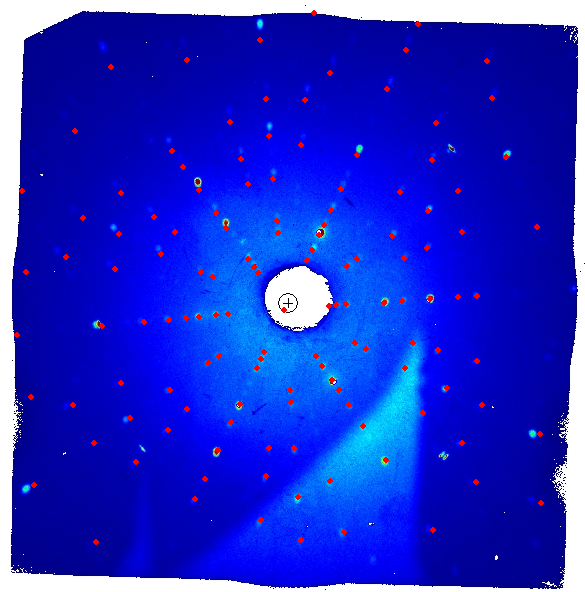
\includegraphics[width=0.6\textwidth]{img_src/Si_laue.png}
    \captionof{figure}{A szilíciumlap kristályrácsának pontjai a Laue-féle röntgendiffrakciós felvételen. Az OrientExpress által kiszámított rácspontok pozícióját piros pöttyök jelképezik.} \label{fig:1}
\end{center}
\begin{center}
    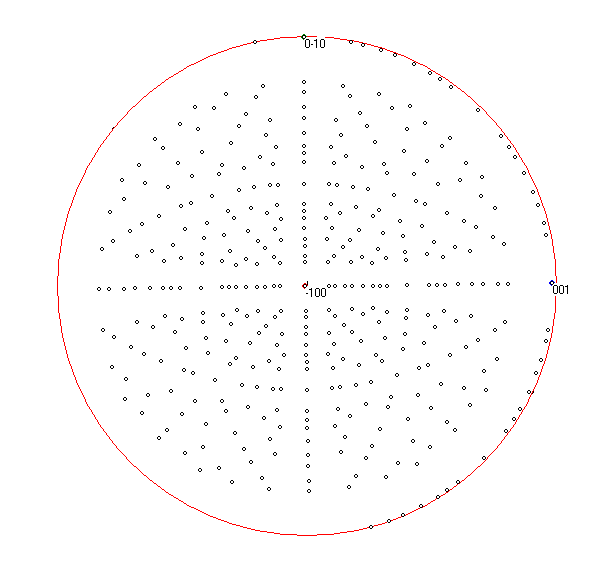
\includegraphics[width=0.6\textwidth]{img_src/Si_stereo.png}
    \captionof{figure}{A szilíciumlap kristályrácsának pontjai sztereografikus projekcióban ábrázolva. A koordináta-rendszer két tengelye a kép síkjával párhuzamos, míg a harmadik azzal merőleges irányba van elforgatva.} \label{fig:2}
\end{center}
\vspace*{\fill}
\newpage
\topskip0pt
\vspace*{\fill}
\begin{center}
    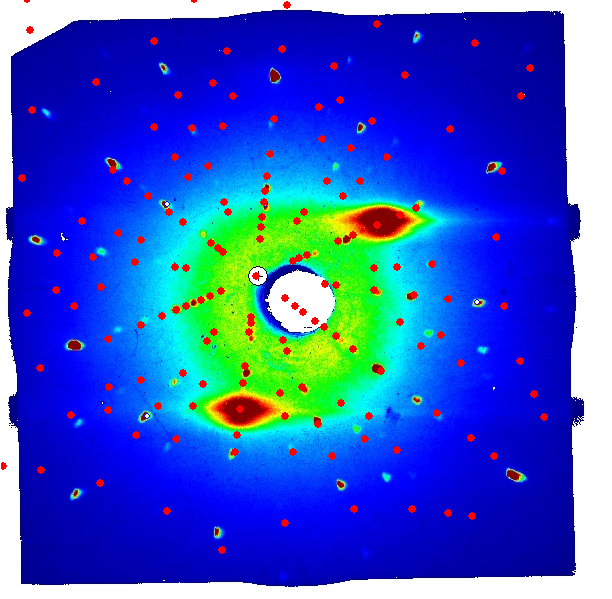
\includegraphics[width=0.6\textwidth]{img_src/diam_laue.png}
    \captionof{figure}{A gyémánt kristályrácsának pontjai a Laue-féle röntgendiffrakciós felvételen. Az OrientExpress által kiszámított rácspontok pozícióját piros pöttyök jelképezik.} \label{fig:3}
\end{center}
\begin{center}
    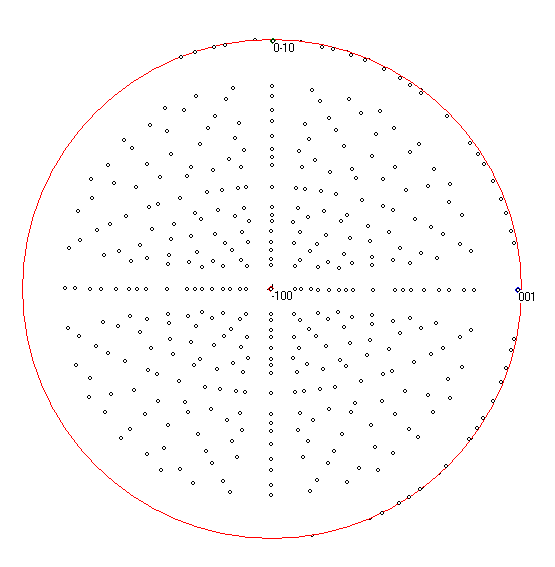
\includegraphics[width=0.6\textwidth]{img_src/diam_stereo.png}
    \captionof{figure}{A gyémánt kristályrácsának pontjai sztereografikus projekcióban ábrázolva. A koordináta-rendszer két tengelye a kép síkjával párhuzamos, míg a harmadik azzal merőleges irányba van elforgatva.} \label{fig:4}
\end{center}
\vspace*{\fill}
\newpage
\topskip0pt
\vspace*{\fill}
\begin{center}
    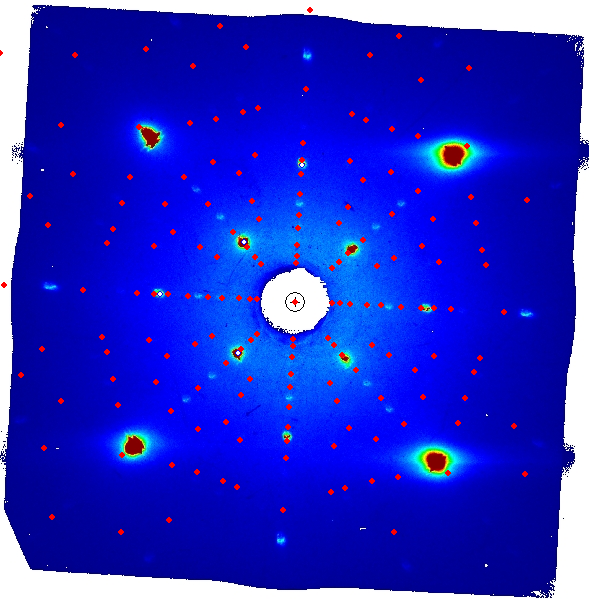
\includegraphics[width=0.6\textwidth]{img_src/NaCl_laue.png}
    \captionof{figure}{A sókristály rácsának pontjai a Laue-féle röntgendiffrakciós felvételen. Az OrientExpress által kiszámított rácspontok pozícióját piros pöttyök jelképezik.} \label{fig:5}
\end{center}
\begin{center}
    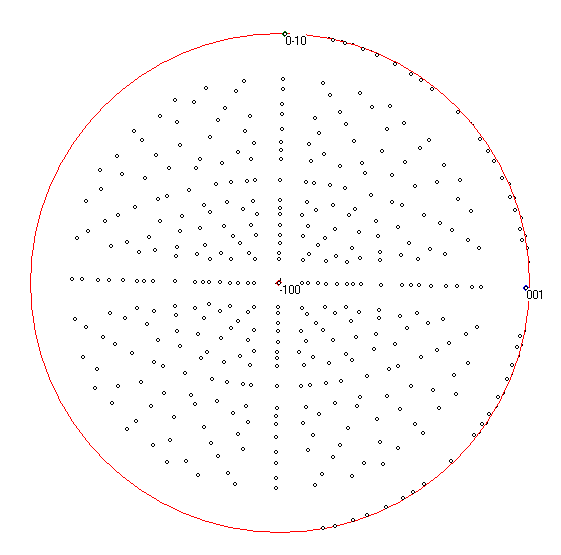
\includegraphics[width=0.6\textwidth]{img_src/NaCl_stereo.png}
    \captionof{figure}{A sókristály rácsának pontjai sztereografikus projekcióban ábrázolva. A koordináta-rendszer két tengelye a kép síkjával párhuzamos, míg a harmadik azzal merőleges irányba van elforgatva.} \label{fig:6}
\end{center}
\vspace*{\fill}